
\documentclass[a4paper]{article}
\usepackage{ucs}  % unicode
\usepackage[utf8x]{inputenc}
\usepackage[T2A]{fontenc}
\usepackage[bulgarian]{babel}
\usepackage{graphicx}
\usepackage{fancyhdr}
\usepackage{lastpage}
\usepackage{listings}
\usepackage{fancyvrb}
\usepackage[usenames,dvipsnames]{color}
\setlength{\headheight}{12.51453pt}

%%%%%%%%%%%%%% Pygments header.
\makeatletter
\def\PY@reset{\let\PY@it=\relax \let\PY@bf=\relax%
    \let\PY@ul=\relax \let\PY@tc=\relax%
    \let\PY@bc=\relax \let\PY@ff=\relax}
\def\PY@tok#1{\csname PY@tok@#1\endcsname}
\def\PY@toks#1+{\ifx\relax#1\empty\else%
    \PY@tok{#1}\expandafter\PY@toks\fi}
\def\PY@do#1{\PY@bc{\PY@tc{\PY@ul{%
    \PY@it{\PY@bf{\PY@ff{#1}}}}}}}
\def\PY#1#2{\PY@reset\PY@toks#1+\relax+\PY@do{#2}}

\def\PY@tok@gd{\def\PY@tc##1{\textcolor[rgb]{0.63,0.00,0.00}{##1}}}
\def\PY@tok@gu{\let\PY@bf=\textbf\def\PY@tc##1{\textcolor[rgb]{0.50,0.00,0.50}{##1}}}
\def\PY@tok@gt{\def\PY@tc##1{\textcolor[rgb]{0.00,0.25,0.82}{##1}}}
\def\PY@tok@gs{\let\PY@bf=\textbf}
\def\PY@tok@gr{\def\PY@tc##1{\textcolor[rgb]{1.00,0.00,0.00}{##1}}}
\def\PY@tok@cm{\let\PY@it=\textit\def\PY@tc##1{\textcolor[rgb]{0.25,0.50,0.50}{##1}}}
\def\PY@tok@vg{\def\PY@tc##1{\textcolor[rgb]{0.10,0.09,0.49}{##1}}}
\def\PY@tok@m{\def\PY@tc##1{\textcolor[rgb]{0.40,0.40,0.40}{##1}}}
\def\PY@tok@mh{\def\PY@tc##1{\textcolor[rgb]{0.40,0.40,0.40}{##1}}}
\def\PY@tok@go{\def\PY@tc##1{\textcolor[rgb]{0.50,0.50,0.50}{##1}}}
\def\PY@tok@ge{\let\PY@it=\textit}
\def\PY@tok@vc{\def\PY@tc##1{\textcolor[rgb]{0.10,0.09,0.49}{##1}}}
\def\PY@tok@il{\def\PY@tc##1{\textcolor[rgb]{0.40,0.40,0.40}{##1}}}
\def\PY@tok@cs{\let\PY@it=\textit\def\PY@tc##1{\textcolor[rgb]{0.25,0.50,0.50}{##1}}}
\def\PY@tok@cp{\def\PY@tc##1{\textcolor[rgb]{0.74,0.48,0.00}{##1}}}
\def\PY@tok@gi{\def\PY@tc##1{\textcolor[rgb]{0.00,0.63,0.00}{##1}}}
\def\PY@tok@gh{\let\PY@bf=\textbf\def\PY@tc##1{\textcolor[rgb]{0.00,0.00,0.50}{##1}}}
\def\PY@tok@ni{\let\PY@bf=\textbf\def\PY@tc##1{\textcolor[rgb]{0.60,0.60,0.60}{##1}}}
\def\PY@tok@nl{\def\PY@tc##1{\textcolor[rgb]{0.63,0.63,0.00}{##1}}}
\def\PY@tok@nn{\let\PY@bf=\textbf\def\PY@tc##1{\textcolor[rgb]{0.00,0.00,1.00}{##1}}}
\def\PY@tok@no{\def\PY@tc##1{\textcolor[rgb]{0.53,0.00,0.00}{##1}}}
\def\PY@tok@na{\def\PY@tc##1{\textcolor[rgb]{0.49,0.56,0.16}{##1}}}
\def\PY@tok@nb{\def\PY@tc##1{\textcolor[rgb]{0.00,0.50,0.00}{##1}}}
\def\PY@tok@nc{\let\PY@bf=\textbf\def\PY@tc##1{\textcolor[rgb]{0.00,0.00,1.00}{##1}}}
\def\PY@tok@nd{\def\PY@tc##1{\textcolor[rgb]{0.67,0.13,1.00}{##1}}}
\def\PY@tok@ne{\let\PY@bf=\textbf\def\PY@tc##1{\textcolor[rgb]{0.82,0.25,0.23}{##1}}}
\def\PY@tok@nf{\def\PY@tc##1{\textcolor[rgb]{0.00,0.00,1.00}{##1}}}
\def\PY@tok@si{\let\PY@bf=\textbf\def\PY@tc##1{\textcolor[rgb]{0.73,0.40,0.53}{##1}}}
\def\PY@tok@s2{\def\PY@tc##1{\textcolor[rgb]{0.73,0.13,0.13}{##1}}}
\def\PY@tok@vi{\def\PY@tc##1{\textcolor[rgb]{0.10,0.09,0.49}{##1}}}
\def\PY@tok@nt{\let\PY@bf=\textbf\def\PY@tc##1{\textcolor[rgb]{0.00,0.50,0.00}{##1}}}
\def\PY@tok@nv{\def\PY@tc##1{\textcolor[rgb]{0.10,0.09,0.49}{##1}}}
\def\PY@tok@s1{\def\PY@tc##1{\textcolor[rgb]{0.73,0.13,0.13}{##1}}}
\def\PY@tok@sh{\def\PY@tc##1{\textcolor[rgb]{0.73,0.13,0.13}{##1}}}
\def\PY@tok@sc{\def\PY@tc##1{\textcolor[rgb]{0.73,0.13,0.13}{##1}}}
\def\PY@tok@sx{\def\PY@tc##1{\textcolor[rgb]{0.00,0.50,0.00}{##1}}}
\def\PY@tok@bp{\def\PY@tc##1{\textcolor[rgb]{0.00,0.50,0.00}{##1}}}
\def\PY@tok@c1{\let\PY@it=\textit\def\PY@tc##1{\textcolor[rgb]{0.25,0.50,0.50}{##1}}}
\def\PY@tok@kc{\let\PY@bf=\textbf\def\PY@tc##1{\textcolor[rgb]{0.00,0.50,0.00}{##1}}}
\def\PY@tok@c{\let\PY@it=\textit\def\PY@tc##1{\textcolor[rgb]{0.25,0.50,0.50}{##1}}}
\def\PY@tok@mf{\def\PY@tc##1{\textcolor[rgb]{0.40,0.40,0.40}{##1}}}
\def\PY@tok@err{\def\PY@bc##1{\fcolorbox[rgb]{1.00,0.00,0.00}{1,1,1}{##1}}}
\def\PY@tok@kd{\let\PY@bf=\textbf\def\PY@tc##1{\textcolor[rgb]{0.00,0.50,0.00}{##1}}}
\def\PY@tok@ss{\def\PY@tc##1{\textcolor[rgb]{0.10,0.09,0.49}{##1}}}
\def\PY@tok@sr{\def\PY@tc##1{\textcolor[rgb]{0.73,0.40,0.53}{##1}}}
\def\PY@tok@mo{\def\PY@tc##1{\textcolor[rgb]{0.40,0.40,0.40}{##1}}}
\def\PY@tok@kn{\let\PY@bf=\textbf\dthod of a LatexFormatter returns a string containing \def commands ef\PY@tc##1{\textcolor[rgb]{0.00,0.50,0.00}{##1}}}
\def\PY@tok@mi{\def\PY@tc##1{\textcolor[rgb]{0.40,0.40,0.40}{##1}}}
\def\PY@tok@gp{\let\PY@bf=\textbf\def\PY@tc##1{\textcolor[rgb]{0.00,0.00,0.50}{##1}}}
\def\PY@tok@o{\def\PY@tc##1{\textcolor[rgb]{0.40,0.40,0.40}{##1}}}
\def\PY@tok@kr{\let\PY@bf=\textbf\def\PY@tc##1{\textcolor[rgb]{0.00,0.50,0.00}{##1}}}
\def\PY@tok@s{\def\PY@tc##1{\textcolor[rgb]{0.73,0.13,0.13}{##1}}}
\def\PY@tok@kp{\def\PY@tc##1{\textcolor[rgb]{0.00,0.50,0.00}{##1}}}
\def\PY@tok@w{\def\PY@tc##1{\textcolor[rgb]{0.73,0.73,0.73}{##1}}}
\def\PY@tok@kt{\def\PY@tc##1{\textcolor[rgb]{0.69,0.00,0.25}{##1}}}
\def\PY@tok@ow{\let\PY@bf=\textbf\def\PY@tc##1{\textcolor[rgb]{0.67,0.13,1.00}{##1}}}
\def\PY@tok@sb{\def\PY@tc##1{\textcolor[rgb]{0.73,0.13,0.13}{##1}}}
\def\PY@tok@k{\let\PY@bf=\textbf\def\PY@tc##1{\textcolor[rgb]{0.00,0.50,0.00}{##1}}}
\def\PY@tok@se{\let\PY@bf=\textbf\def\PY@tc##1{\textcolor[rgb]{0.73,0.40,0.13}{##1}}}
\def\PY@tok@sd{\let\PY@it=\textit\def\PY@tc##1{\textcolor[rgb]{0.73,0.13,0.13}{##1}}}

\def\PYZbs{\char`\\}
\def\PYZus{\char`\_}
\def\PYZob{\char`\{}
\def\PYZcb{\char`\}}
\def\PYZca{\char`\^}
% for compatibility with earlier versions
\def\PYZat{@}
\def\PYZlb{[}
\def\PYZrb{]}
%%%%%%%%%%%%%% Pygments header end.


\pagestyle{fancy}
%\fancyhead{}
\fancyfoot{}

\cfoot{\thepage\ от \pageref{LastPage}}

\addto\captionsbulgarian{%
  \def\abstractname{%
    Цел на проекта} %\cyr\CYRA\cyrs\cyrt\cyrr\cyra\cyrk\cyrt}}%
}

% VCS = Version Control Systems

% Custom defines:
\def\git{\texttt{git}}
\def\SCM{SCM}
% \def\js{\texttt{javascript}}
% \def\jsg{JsGames}
% \def\jsurl{http://iskren.info:50005/}

% TODO remove colorlinks before printing
\usepackage[unicode,colorlinks]{hyperref}   % this has to be the _last_ command in the preambule, or else - no work
\hypersetup{urlcolor=blue}
\hypersetup{citecolor=PineGreen}

 \begin{document}

\title{Дистрибутирани системи за управление на сорс код}
\author{
Зорница Атанасова Костадинова, 4 курс, КН, фн: 80227, \\
Искрен Ивов Чернев, 4 курс, КН, фн: 80246
}
\date{\today}
\maketitle

%\includegraphics[scale=0.1]{drop}

\begin{abstract}
Да запознае читателя с историята и развитието на системите за управление на код (\SCM). Ще бъдат сравнени централизираните и дистрибутираните системи както на високо ниво - предимства, недостатъци, сфери на приложение - така и на ниско ниво - обща архитектура, представяне на данните, използвани алгоритми и структури от данни. Ще бъде обърнато специално внимание на дистрибутираните системи за управление на код, тъй като те са по-нови като концепция и вече успешно заместват централизираните системи във все повече проекти, най-забележимо тези с отворен код, но също и в големи компании които по исторически причини използват централизирани системи (google, facebook).
\end{abstract}
\newpage

\setcounter{tocdepth}{2}
\tableofcontents
\newpage

%%%%%
%%%%% Templates
%%%%%
% \section{Секция}
% 
% \subsection{Под секция}
% \subsubsection{Под под секция}
% 
% Enumerate list \cite{foo}
% 
% \begin{enumerate}
%   \item първо
%   \item второ
%   \item трето
% \end{enumerate}
% 
% Itemize list
% 
% \begin{itemize}
%   \item Едно
%   \item[Две] 2
%   \item[Триииииииииииииииииииииииииии] три три три три три
%   три три три три
% \end{itemize}
% 
% Description list
% 
% \begin{description}
%   \item[Foo] bar
%   \item[баз] quux
% \end{description}

%%%%%% Begin of document (BOD)

\section{Увод}
Системите за управление на код (\SCM) играят важна роля в процеса на
разработване на софтуер. Те съхраняват историята на развитие на файловете като
по този начин позволяват на потребителя да прегледа направените промени по
различни критерии (времеви период, потребител направил промяната и др.).
Правенето на промени по кодовата база също е благоприятствано от факта, че
винаги може да се игнорират и състоянието на проекта да бъде върнато към
по-старо и стабилно състояние. Историята на развитие на проекта може да бъде
използвана и от хора интересуващи се от прогреса по проекта (мениджъри,
клиенти), с цел създаване на план за по-нататъшно развитие, оценка за свършена
работа и други.


Софтуерните проекти обикновено се развиват в няколко направления:
\begin{itemize}
  \item едно или няколко стабилни направления - използват се от обикновения
  потребител;
  \item направление за тестване (beta версия) - използват се от по-напреднали
  потребители, които искат да получат нововъведенията колкото се може по-скоро,
  на цената на по-нестабилно изпълнение;
  \item направление за развитие - използва се от програмистите докато
  разработват най-новите промени по кода.
\end{itemize}


\SCM\ предоставят възможности за управление на отделните направление, като по
този начин може да се разграничи кои версии от историческото развитие се
използват от програмисти, тестери и обикновени потребители.

\section{История и развитие на \SCM}
Нуждата от \SCM\ се появява през 60\textsuperscript{те} и
70\textsuperscript{те} години на XX век. През
това време се появяват първите по-големи софтуерни проекти и става ясно, че
поддържането на историята на развитие на проекта е крайно наложително.
Развитието преминава през няколко периода:
  \subsection{Ръчно управление}
  В началото всеки сам е решавал проблема с пазене на история на проект или
  отделен файл. Нужен е бил механизъм за запаметяване на състоянието на един
  или няколко файла в един момент, за да може при нужда да се върне старо
  състояние. Това може да става със запазване на стара версия на файла с
  различно разширение (например \texttt{filename.old.1},
  \texttt{filename.old.2} и т.н.) или създаване на архив на цяла директория.
  Тези подходи вършат работа при малки начинания, но имат големия недостатък че
  изразходват много памет. Ако един файл има дължина 1 Kb, и е бил запазен 20
  пъти по време на своето създаване, тогава заеманата памет е приблизително
  $1000 * 20 / 2 = 10 \mathrm{Kb}$. Това означава, че заеманата памет нараства
  линейно с нарастването на запаметените ревизии. На практика обаче, всяка
  ревизия се различава с малко от предходната, т.е. заеманата памет теоретично
  може да бъде пропорционална само на размера на проекта, независимо от броя на
  ревизиите.

  \subsection{Локално управление}
  Първите софтуерни продукти за управление на код са работели на ниво отделен
  файл. Т.е. те са запазвали историята на един файл независимо от останалите.
  Това може да бъде постигнато като за всяка нова ревизия бъде запазена
  разликата с предишната. Първата система, която реализира това е
  SCCS\cite{sccs}. Тя използва формата припокриващи се разлики (interleaved
  deltas) за да запазва различията между версиите на един файл. Системата е
  била разработвана от Bell Labs и се разпространявала чрез заплащане.
  RCS\cite{rcs} е наследник на SCCS и набрала голяма популярност през
  80\textsuperscript{те} години, защото била безплатен и развит еквивалент на
  SCCS. RCS също предоставяла възможност за следене на история на всеки файл по
  отделно. Освен работната версия на файла се пазел и файл с историята,
  съдържащ списък с различията еволюирали файла от началното до крайното му
  състояние.

  \subsection{Централизирано управление}
  Системите до момента предоставят възможност за пазене на историята на отделни
  файлове на компютъра на който са били създадени. Често тази история е
  трябвало да се споделя между група хора - например екип програмисти.
  Дистрибутирането на файла с историята между няколко компютъра се оказала
  не-тривиална задача, особено при наличието на много файлове. Нужна била
  система, която е в състояние да управлява всички файлове на проекта и да
  осигури лесен и бърз начин за достъпване на историята на проекта от всеки
  член на екипа. С тези идеи бил създаден CVS\cite{cvs} - една от
  най-известните системи за управление на код, използвана и в момента от
  немалко проекти. В нея било имплементирано запазването на история за всеки
  файл, точно както RCS както и централен сървър на който стояла информация за
  историята на всички файлове. Всеки клиент пазел само една текуща версия на
  всички файлове и при нужда от други версии се свързвал със сървъра и изтеглял
  нужната му информация. За да поправи много от проблемите открити с времето в
  CVS бил създаден Subversion\cite{svn}. Subversion има мото "CVS направен
  както трябва". Тъй като наистина решавал практични проблеми, налични в CVS, а
  също бил изключително лесен за използване много проекти използващи CVS
  преминават на Subversion. При Subversion се запазва идеята за централен
  сървър, на който стои цялата история на всички файлове като при нужда
  клиентите изтеглят нужната им информация.

  \subsection{Дистрибутирано управление}
  Дистрибутираните системи за управление на код приличат на централизирана
  система, при която всеки клиент пази пълната история на развитие на проекта.
  Тъй като всеки клиент държи пълно копие на историята и добавя сам нова
  история трябва да съществува механизъм за обмяна на промените направени между
  два клиента. Това означава, че може да се симулира модела на работа на
  централизираните системи като се избере един централен клиент и всички
  останали синхронизират с него. На практика се използва както централен
  клиент, така и синхронизиране на два нецентрални клиента, в зависимост от
  ситуацията. Най-видните примери за дистрибутирани системи за управление са
  Git\cite{git} и Mercurial\cite{mercurial}. Те набират голяма популярност сред
  опън сорс обществото, защото позволяват по естествен начин да се споделят
  промени направени от хора, който не се познават предварително и следователно
  няма как да споделят общ централен сървър.

\section{Сравнение на архитектурно ниво}
  \subsection{Архитектура на централизираните системи}
    \subsubsection{Архитектура на CVS}
    \subsubsection{Архитектура на Subversion}
    
    Apache Subversion (или само SVN по името на командата svn) е система за контрол на версиите създадена с цел да бъде силно подобна на CVS, поправяйки грешките и имплементирайки някои липсващи нейни функционалности. Използва се широко в средите почитащи отворения код. Сред примерите са Apache Software Foundation, FreeBSD, GCC, Django, Ruby, Tigris.org, PHP, Python и MediaWiki. Google Code и SourceForge предоставят Subversion хостинг за проекти с отворен код.

    Функционалности, които го правят предпочитан пред CVS:
    \begin{itemize}
      \item \texttt{Атомарни commit'и} - В смисъла на транзакциите. Или цялото множество от промени се регистрира, или абсолютно нищо.
      \item \texttt{Пълна история} на преименовани, копирани или преместени файлове и директории.
      \item \texttt{Метаданни} - Може да се съхранява информация за файлове и директории под формата на двойки ключ - стойност.
      \item \texttt{Двоични файлове} - Съхранението им е ефективно, като от ревизия до ревизия се пази само binary-diff.
      \item \texttt{Branching} e евтина операция независеща от размера на файловете. Механизмът е подобен на хард-линковете в UNIX.
      \item \texttt{Обмен на малко информация} - Протоколът между клиента и сървъра изпраща само diff'ове на файловете в двете посоки.
      \item \texttt{Резултатите} са удобни за парсене. Има възможност за получаване на лог във вид на XML.
      \item \texttt{Конфликти} - За да се избегне необходимостта от разрешаване на конфликти, файловете могат да се заключват. Така програмистът си запазва ексклузивното право само той да ги редактира (reserved checkout).
      %\item Path-based authorization.
      \item \texttt{Интеграция} - SVN е написан на C, но поддържа интеграция също със C\#, PHP, Python, Perl, Ruby и Java.
    \end{itemize}

    \paragraph{Архитектура}
    Моделът е клиент-сървър, дизайнът на библиотеките е слоест.

    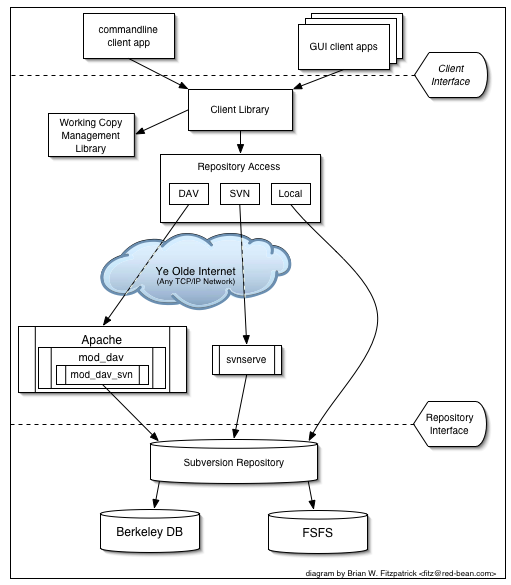
\includegraphics[scale=0.5]{svn_architecture}

    В долната част на схемата се намира SVN repository \textsuperscript{то} което съдържа всички данни, които са регистрирани за контрол на версиите. В горната част е представена клиентската програма която управялва локалните копия на тези данни (наречени работни копия). Помежду им са множество маршрути през различни слоеве за достъп до repository. Някои от тях минават през мрежата и през сървъри, които от своя страна достъпват repo \textsuperscript{то}. Други заобикалят мрежата и директно достъпват repository \textsuperscript{то}. 

    \paragraph{Видове хранилища}

    \begin{itemize}
      \item \texttt{Berkeley DB}
      \item \texttt{FSFS} - Предпочитаният метод за съхраниение на данните, тъй като работи по-бързо и заема по-малко място на диска.
    \end{itemize}

    \paragraph{Достъп до хранилищата}

    \begin{itemize}
      \item \texttt{Местна или мрежова файлова система} - Използва протокола file:///path.
      \item \texttt{WebDAV / Delta-V} - Чрез модула mod\_dav\_svn за Apache. Протоколът е http(s).
      \item \texttt{Специализиран svn протокол} - Предава обикновен текст (svn://host/path) или криптиран през ssh (svn+ssh://host/path).
    \end{itemize}

    \paragraph{Клиенти}

    \begin{itemize}
      \item В командния ред
        \begin{itemize}
          \item Subversion предоставя собствен клиент за командния ред.
        \end{itemize}
      \item В мениджъра на прозорците
        \begin{itemize}
          \item TortoiseSVN е разширение на Windows shell\textsuperscript{а} което информира за състянието на файловете в revision системата като модифицира иконите в Windows Explorer.
          \item SmartSVN работи на подобен принцип.
        \end{itemize}
      \item Интегрирани в средата за разработване на код
        \begin{itemize}
          \item AnkhSVN е предвидена за ползване с Microsoft Visual Studio.
          \item Subclipse, Subversive работят заедно с Eclipse.
          \item Xcode е редактор, включен в Mac OS X 10.5 (Leopard), поддържащ SVN.
        \end{itemize}
      \item Уеб-базирани
        \begin{itemize}
          \item Trac - вдъхновена е от CVSTrac и първоначално е наречена ``svntrac'' заради интеграцията си със Subversion.
        \end{itemize}
    \end{itemize}

    \paragraph{Слоеве}

    \begin{itemize}
      \item \texttt{Файлова система} - Това е най-ниското ниво на което се съхраняват потребителските данни.
    The lowest level; it implements the versioned filesystem which stores the user data.
      \item \texttt{Хранилища} - Контролира скриптовете които изпълняват действията по контрол на версиите. Тези два слоя заедно съставялват интерфейса на файловата система.
      \item \texttt{mod\_dav\_svn} - Осигурява WebDAV / Delta-V достъп чрез Apache 2.
      \item \texttt{Достъп до хранилището} - Този слой контролира както местния така и отдалечения достъп. На това ниво към хранилищата се обръщаме чрез URL:
        \begin{itemize}
          \item \texttt{местен достъп}: file:///path/
          \item \texttt{WebDAV}: http://host/path/; https://host/path/
          \item \texttt{протокол SVN}: svn://host/path/; svn+ssh://host/path/
        \end{itemize}
      \item \texttt{Клиент, Работно копие на проекта} - Най-високото ниво абстрахира достъпа до кранилището и предоставя интерфейс за общи клиентски задачи като автентикация на потребители и сравнение на версии.
    \end{itemize}

  \subsection{Архитектура на дистрибутираните системи}
    \subsubsection{Архитектура на Mercurial}
    \subsubsection{Архитектура на Git}

\section{Сравнение на функционално ниво}
  \subsection{Предимства на централизираните системи}
  \subsection{Недостатъци на централизираните системи}
  \subsection{Предимства на дистрибутираните системи}
  \subsection{Недостатъци на дистрибутираните системи}

\section{Заключение}

%%%%%% End of document (EOD)
\newpage

\begin{thebibliography}{99}
  \bibitem{foo} \url{http://example.com/}
  \bibitem{sccs} \url{http://sccs.berlios.de/}
  \bibitem{rcs} \url{http://www.gnu.org/software/rcs/}
  \bibitem{cvs} \url{http://savannah.nongnu.org/projects/cvs}
  \bibitem{svn} \url{http://subversion.apache.org/}
  \bibitem{git} \url{http://git-scm.com/}
  \bibitem{mercurial} \url{http://mercurial.selenic.com/}
  \bibitem{git-bottom-up}
  \url{http://ftp.newartisans.com/pub/git.from.bottom.up.pdf}
\end{thebibliography}

\end{document}
